% --------------------------------------------------------------------------
% Template for WASPAA-2025 paper; to be used with:
%          waspaa25.sty - WASPAA 2025 LaTeX style file,
%          IEEEtran.cls - IEEE Transactions class file, and
%          IEEEtran.bst - IEEE Transactions bibliography style file.
%
% --------------------------------------------------------------------------

\documentclass[9pt,conference]{IEEEtran}
%% For double-blind submission, use this:
% \usepackage[doubleblind]{waspaa25}

%% For camera-ready version, use this:
% \usepackage{waspaa25} % removes hyperlinks (required by IEEE Xplore)

%% If you need a preprint version with authors/affiliations and hyperlinks:
\usepackage[preprint]{waspaa25}

\usepackage{bm} % for bold math symbols (incl. Greek letters) with \bm{}


% Example definitions.
% --------------------
\newcommand{\RR}{\mathbb{R}}

% Title.
% --------------------
\title{Toward a Sparse Interpretable Audio Codec}

%%%%%%%%%%%%%%%%%%%%%%%%%%%%%%%%%%%%%%%%%%%%%%%%%%%%%%%%%%%%%%%
%%  Please use the commands below to include author          %%
%%  information for the camera-ready/preprint versions.      %%
%%  The information is obfuscated in the review version.     %%
%%%%%%%%%%%%%%%%%%%%%%%%%%%%%%%%%%%%%%%%%%%%%%%%%%%%%%%%%%%%%%%

\name{John Vinyard}
\address{
  1401 O K Corral, Austin TX, USA \\
  \href{mailto:john.vinyard@gmail.com}{john.vinyard@gmail.com}
}


\begin{document}

\maketitle

\begin{abstract}
  Most widely-used modern audio codecs, such as Ogg Vorbis and MP3, as well as more recent ``neural'' codecs like Meta's Encodec or Descript's are based on block-coding; audio is divided into overlapping, fixed-size ``frames'' which are then compressed. While they result in excellent reproduction quality and can be used for downstream tasks such as text-to-audio, they do not produce an intuitive, directly-interpretable representation.
  In this work, we introduce a proof-of-concept audio encoder that represents audio as a sparse set of events and their times-of-occurrence. Rudimentary physics-based assumptions are used to model attack and the physical resonance of both the instrument being played and the room in which a performance occurs, hopefully encouraging a sparse, parsimonious, and easy-to-interpret representation.
\end{abstract}


\section{Introduction}
\label{sec:intro}

We imagine a near-future audio codec where some types of musical composition could take place directly in the audio codec space. Text-to-audio is an excellent interface for non-musicians creating background music for movies, advertisements or social media content, but it is our view that experienced musicians and composers work in a "space" not fully captured by language and will prefer a much finer-grained representation that affords an effectively infinite range of possible sounds.

This work clearly does not replace current music generation models, but could serve as the underlying encoding on which generative models are trained. It is the authors' intuition that models trained on this rich, symbolic representation might have a much deeper "understanding" of the content they produce, given the point-cloud-like nature of the signal. Instead of predicting the next frame, the generative model would be predicting the relationships between "events". Long-term coherence in musical generation has always been a difficult problem, and we speculate that many models spend enormous shares of their capacity learning to reproduce physical resonance, rather than the human forces that drive them in interesting, musical directions.

All model and experiment code is written in PyTorch and 
can be found on GitHub\footnote{\href{https://github.com/JohnVinyard/matching-pursuit}{https://github.com/JohnVinyard/matching-pursuit}}. 
Audio examples can be heard at this https URL\footnote{\href{https://blog.cochlea.xyz/sparse-interpretable-audio-codec-paper.html}{https://blog.cochlea.xyz/sparse-interpretable-audio-codec-paper.html}}

\section{Prior Work}
\label{sec:prior_work}


This work draws inspiration from a number of existing techniques, including the field of Auditory Scene Analysis and blind source separation, as well as machine learning techniques like matching pursuit and synthesis techniques like granular synthesis.

- auditory scene analysis
- audio source separation
- granular synthesis
- matching pursuit
- source-excitation models (NEEDS A REFERENCE)

\section{Data Set}
\label{sec:data_set}

We train our model on the MusicNet dataset \cite{thickstun2017learning}, an open dataset containing 33 hours 
of classical music, recorded in diverse spaces using a range of 
recording equipment of varying quality.  The recordings often include leading 
silence, trailing applause, and incidental human sounds throughout 
(coughs, movement, etc).




\section{Model}
\label{sec:model}

\subsection{Encoder}
\label{ssec:encoder}

Inspired by matching pursuit, the encoding process is iterative, or incremental.
At each step, the encoder chooses a single event vector and time-of-occurrence and passes this
to the decoder, which generates and schedules audio and subtracts it from the input representation.  This process
is repeated for some fixed number of steps or until some stopping condition is reached.

The encoder is paramaterized as an anti-causal, dilated convolutional network.

% Below is an example of how to insert images.
% -------------------------------------------------------------------------
\begin{figure}[t]
  \centering
  \centerline{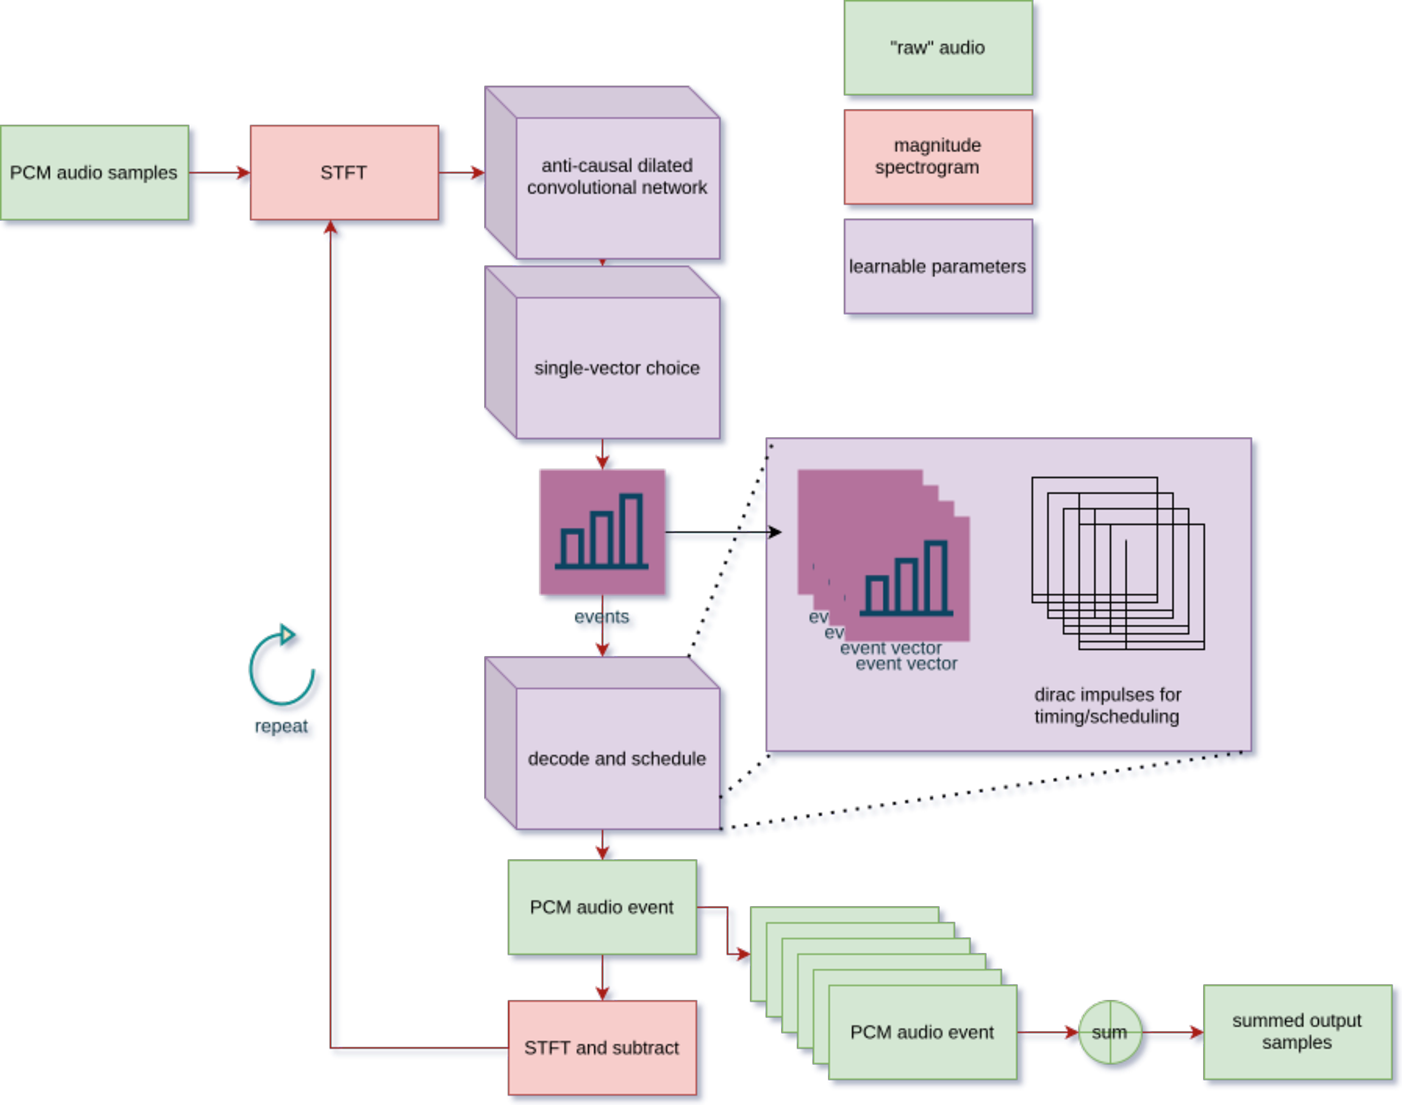
\includegraphics[width=\columnwidth]{model}}
  \caption{Model architecture}
  \label{fig:model_architecture}
\end{figure}


\subsection{Decoder}
\label{ssec:decoder}

TODO: Diagram of decoder block and scheduling process

\section{Experiments}
\label{sec:experiments}

\section{Interpretable and Manipulatable Representation}
\label{sec:interpretable_representation}


\section{Future Work}
\label{sec:future_work}

\section{Double-Blind Review}
\label{sec:double_blind}

This year's review process will again be double-blind, without any blackout period (authors are free to release their work on arXiv and advertise it on social media if they so choose). 

It is imperative that the authors ensure that they do not reveal their identity and affiliation in their manuscript. The manuscript submission should be prepared using \texttt{\textbackslash{}usepackage[doubleblind]\{waspaa25\}}, which will automatically remove the author and affiliation information. 

To produce the camera-ready version if the paper is accepted, please use \texttt{\textbackslash{}usepackage\{waspaa25\}} instead. This will include author and affiliation information and remove hyperlinks, as required by IEEE Xplore.

If you need a preprint version that includes author and affiliation information and retains hyperlink ({\bf not for camera-ready!}), please use \texttt{\textbackslash{}usepackage[preprint]\{waspaa25\}}.

\section{Important remark regarding this template}
\label{sec:new_template}

This new \LaTeX\ template is by default much tighter and more compact than previous WASPAA or ICASSP templates. Vertical spacing around sections, subsections, equations, figures, tables, and captions was tuned to be already quite small by default, and we thus highly discourage the use of \texttt{\textbackslash{vspace}}. 

\section{Formatting your paper}
\label{sec:format}

All manuscripts must be submitted electronically as PDF files.
All manuscripts must be formatted for white US letter paper
(8.5 $\times$ 11 inches). Please do {\bf not} use A4-size papers.
All printed material, including text, illustrations, and charts, must be kept within a print area of 7.14 inches (181.35 mm) wide by 9.32 inches (236.85 mm) high. Do not write or print anything outside the print area. The top margin from the edge of the paper to the top of a capital T on the first line of text must be 0.71 inch (18.1 mm), except for the title page (see \cref{sec:pagestyle}, the bottom margin must be 1.05 inch (26.6 mm), the left and right margin must be 0.68 inch (17.3 mm). All {\it text} must be in a two-column format. Columns are to be 3.487 inches (88.57 mm) wide, with a 0.166 inch (4.22 mm) space between them. Text must be fully justified.


\section{PDF EXPRESS}
\label{sec:PDF_express}

Accepted papers must pass the IEEE PDF Express$^{\text{TM}}$ format verification prior to publication \cite{IEEEXploreReqs}. Format verification details will be announced with the paper acceptance notification.

\section{Electronic Copyright Form}
\label{sec:copyright}

You will be requested to sign an IEEE Electronic Copyright Form after your manuscript is selected for presentation at the workshop. This form {\bf must} be submitted before your paper can be published in the proceedings. 
Electronic copyright form submission details will be announced with the paper acceptance notification.

\section{Number of Pages}
\label{sec:pagelimit}

You are allowed a total of 5 pages for your document. Up to 4 pages may
contain technical content, figures, and references, while the 5th page
may contain only references. This is the maximum number of pages that
will be accepted, including all figures, tables, and references. Any document that exceeds the 5-page limit will be rejected. Any document
with a 5th page containing anything other than references will be rejected.


\section{Page Title Section}
\label{sec:pagestyle}

The paper title (on the first page) should begin 0.949 inches, or 24.10 mm, from the edge of the page if using 9pt font (0.984 inches, or 25.00 mm, if using 10pt font). It should be centered, in Title Case, and in Times 17-point if using 9pt font (in Times 20-point font if using 10pt font), regular (non-bold) type. The authors' name(s) and affiliation(s) appear below the title in capital and lowercase letters (i.e., with their customary capitalization). The authors' name(s) should be italicized, and the affiliation upright (non-italicized). Papers with multiple authors and affiliations may require two or more lines for this information.

\section{Type-Style and Fonts}
\label{sec:typestyle}

To achieve the best rendering in the proceedings, we strongly encourage you to use Times Roman font. In addition, this will give the proceedings a more uniform look. Use a font that is no smaller than 9pt type (the recommended setting) for the body text. If you wish to use 10pt type font, remove the \texttt{9pt} option when loading the document class. Note that the abstract, figure captions, and tables are in 8pt font in both cases.

In 9pt type font, capital letters are 2 mm high. {\bf If you use the 9pt size, the interline spacing (i.e., \texttt{\textbackslash{baselineskip}}) should be 3.9 mm (0.153 inch), and there should thus be no more than 2.57 lines/cm (6.54 lines/inch) vertically.} This is a minimum spacing. Larger type sizes require correspondingly larger vertical spacing. Please do not double-space your paper. True-Type 1 fonts are preferred.

The first paragraph in each section should not be indented, but all the following paragraphs within the section should be indented, as these paragraphs demonstrate.

\section{Major Headings}
\label{sec:majhead}

Major headings, for example, ``{\bf 1. INTRODUCTION}'', should appear in all capital letters, bold face, centered in the column. Vertical spacing before the heading should be between 0.055 inches and 0.166 inches in 9pt font, and between 0.062 inches and 0.187 inches in 10pt font; vertical spacing after the heading should be between 0.039 inches and 0.094 inches in 9pt font, and between 0.044 inches and 0.106 inches in 10pt font. Use a period (``.'') after the heading number. Sections can be referenced using \cref{sec:majhead}, \cref{ssec:subhead}, and \cref{sssec:subsubhead}.


\subsection{Subheadings}
\label{ssec:subhead}

Subheadings should appear in lowercase (initial word capitalized) in boldface. They should start at the left margin on a separate line. Vertical spacing before the subheading should be between 0.042 inches and 0.138 inches in 9pt font, and between 0.047 inches and 0.156 inches in 10pt font.

\subsubsection{Sub-subheadings}
\label{sssec:subsubhead}

Sub-subheadings, as in this paragraph, are discouraged. However, if you must use them, they should appear in lower case (initial word capitalized), indented, with the paragraph text following on the same line, after a semi-colon. The sub-subheadings should be in italics.

\subsubsection{Sub-subheadings should never be alone}
\label{sssec:subsubhead2}

There should never be a unique sub-subsection within a subsection.

\subsection{Subheadings also should never be alone}
\label{ssec:subhead2}

There should never be a unique subsection within a section.

\section{Page Numbering}
\label{sec:page}

Please do {\bf not} paginate your paper. Page numbers, session numbers, and conference identification will be inserted when the paper is included in the proceedings.

\section{Figures}
\label{sec:illust}

Since there are many, often incompatible, ways to include images (e.g., with experimental results) in a \LaTeX\ document, an example of how to do
this is presented in \cref{fig:results}. \Cref{fig:results} should be used at the beginning of a sentence, and \cref{fig:results} otherwise.

% Below is an example of how to insert images.
% -------------------------------------------------------------------------
\begin{figure}[t]
  \centering
  \centerline{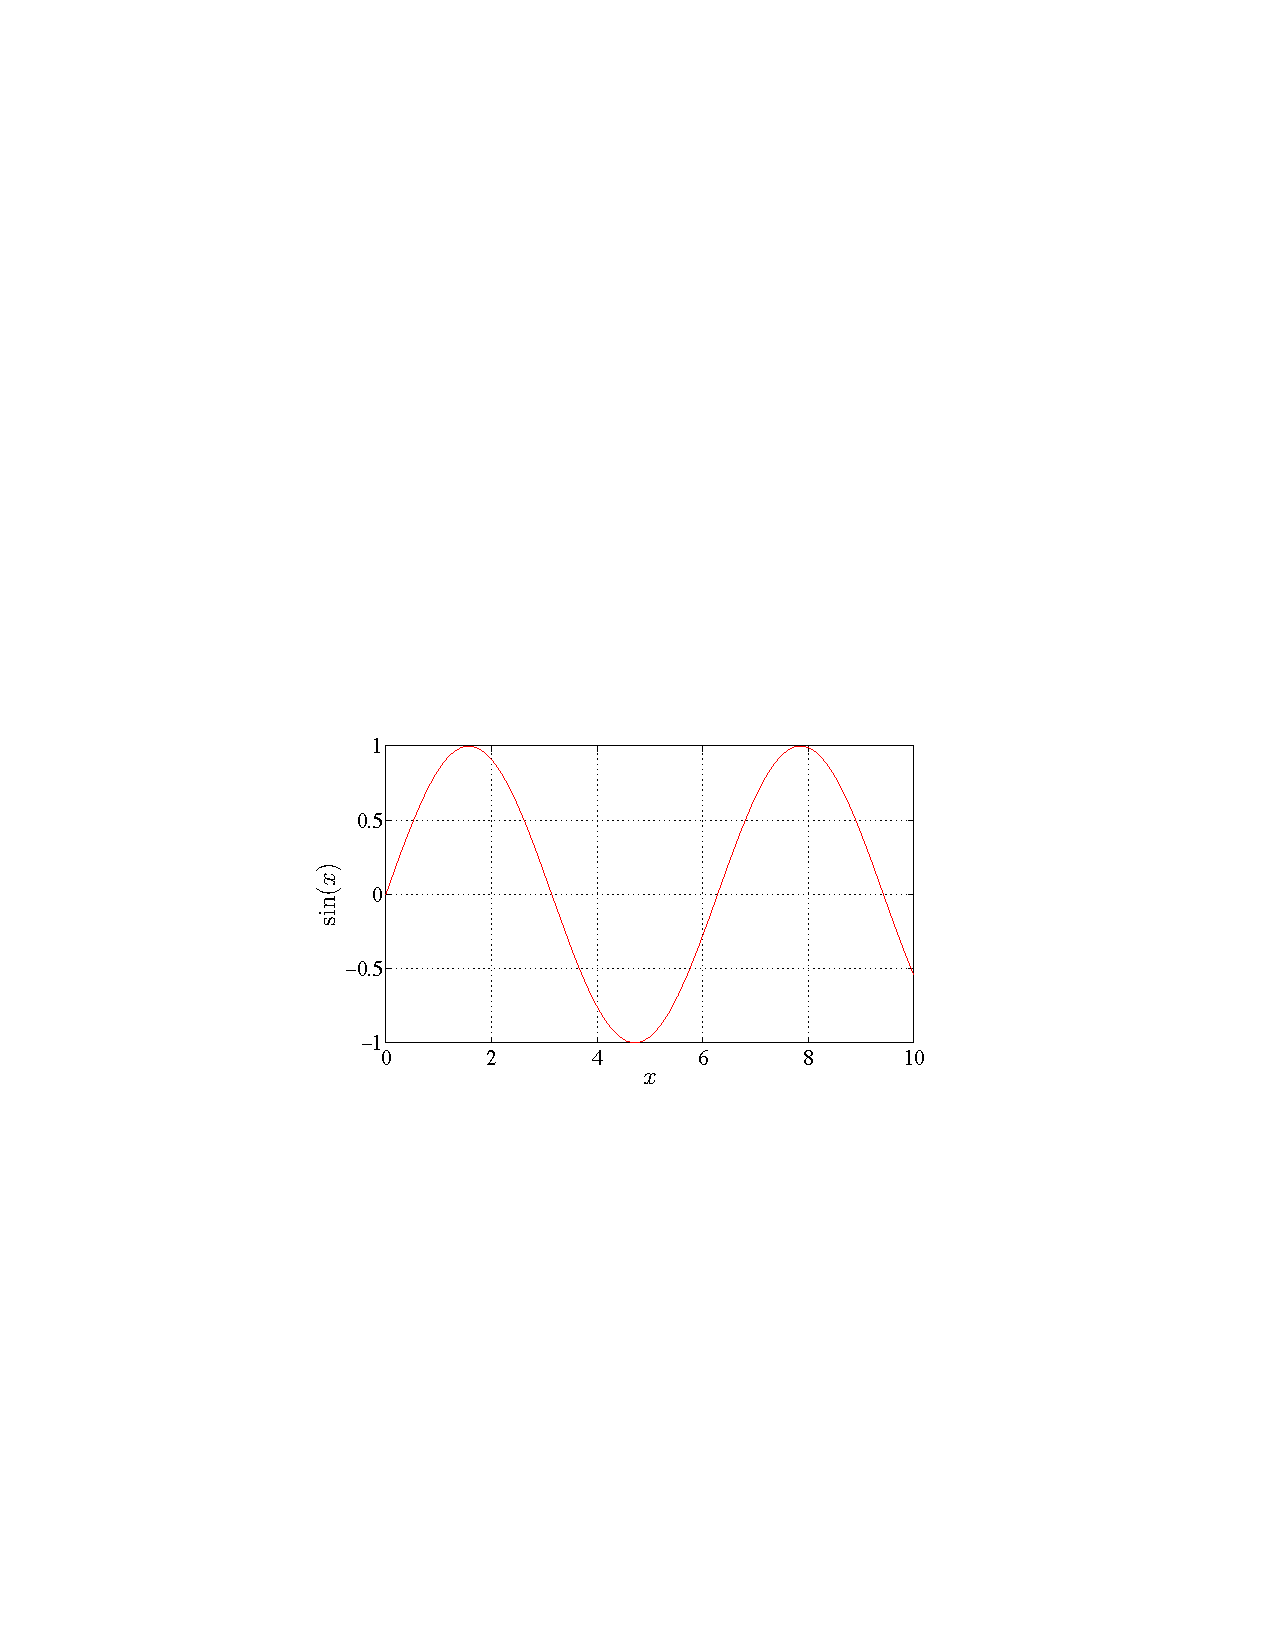
\includegraphics[width=\columnwidth]{fig1}}
  \caption{Example of a figure with experimental results, where the caption is long and wraps on the next line.}
  \label{fig:results}
\end{figure}

When inserting PDFs, we recommend using \texttt{pdfcrop} to remove unnecessary margins. This will allow you to better fine-tune the size of your figure when inserting it with \texttt{\textbackslash{includegraphics}}.

Illustrations must appear within the designated margins. They may span the two columns. If possible, position illustrations at the top of columns, rather than in the middle or at the bottom. Caption and number every illustration. All halftone illustrations must be clear black and white prints. Colors may be used, but they should be selected so as to be readable when printed on a black-only printer, or markers and line styles should be used to make figures readable without relying on colors.



\section{Equations}
\label{sec:equations}

Equations should be placed on separate lines and consecutively numbered with equation numbers in parentheses flush with the right margin, as illustrated in \cref{eq:wave_equation} that gives the homogeneous acoustic wave equation in Cartesian coordinates \cite{eWilliams1999},
\begin{equation}
  \label{eq:wave_equation}
    \Delta^2p(\bm{x},t)-
    \displaystyle\frac{1}{c^2}\frac{\partial^2p(\bm{x},t)}{\partial t^2}=0,
\end{equation}
where $p(\bm{x},t)$ is an infinitesimal variation of acoustic pressure from its equilibrium value at position $\bm{x}\in\RR^3$ and time $t$, and where $c$ denotes the speed of sound.

Symbols in your equation should be defined before the equation appears or immediately following.  Use \cref{eq:wave_equation}, not Eq. (1) or equation (1), except at the beginning of a sentence: ``\Cref{eq:wave_equation} is ...''

\section{Footnotes}
\label{sec:foot}

Use footnotes sparingly\footnote{or not at all!} and place them at the bottom of the column on the page on which they are referenced. Use Times 8-point type, single-spaced. To help your readers, avoid using footnotes altogether and include necessary peripheral observations in the text (within parentheses, if you prefer, as in this sentence).

\section{References}
\label{sec:ref}

List and number all bibliographical references at the end of the paper. The references should be numbered in order of appearance in the document. When referring to them in the text, type the corresponding reference number in square brackets as shown at the end of this sentence \cite{cJones2003,aSmith2000} or \cite{eWilliams1999,cJones2003,aSmith2000}. For \LaTeX\ users, the use of the Bib\TeX\ style file IEEEtran.bst is recommended, which is included in the \LaTeX\ paper kit available from the workshop website \cite{waspaaweb}.

\section{Acknowledgment}
\label{sec:ack}

The preferred spelling of the word acknowledgment in America is without an ``e'' after the ``g.'' Try to avoid the stilted expression, ``One of us (R.\ B.\ G.) thanks ...'' Instead, try ``R.\ B.\ G.\ thanks ...''  Put sponsor acknowledgments in the unnumbered footnote on the first page. Please include acknowledgments only in the camera-ready version, and NOT in the version of the paper submitted for review.

% -------------------------------------------------------------------------
% Either list references using the bibliography style file IEEEtran.bst

\clearpage
% The \IEEEtriggeratref{XX} command can be used to move to the next column before the XX-th reference
% to balance the two columns of the reference section
% \IEEEtriggeratref{XX}
\bibliographystyle{IEEEtran}
\bibliography{refs25}
% or list them by yourself:
% \begin{thebibliography}{1}

% \bibitem{waspaaweb}
% {WASPAA Website}, \url{http://www.waspaa.com}.

% \bibitem{IEEEXploreReqs}
% {IEEE {X}plore {R}equirements}, \url{https://conferences.ieeeauthorcenter.ieee.org/write-your-paper/meet-ieee-xplore-requirements/}.

% \bibitem{eWilliams1999}
% E.~Williams, \emph{Fourier Acoustics: Sound Radiation and Nearfield Acoustic Holography}.\hskip 1em plus 0.5em minus 0.4em\relax London, UK: Academic Press, 1999.

% \bibitem{cJones2003}
% C.~Jones, A.~Smith, and E.~Roberts, ``A sample paper in conference proceedings,'' in \emph{Proc. ICASSP}, vol.~II, Apr. 2003, pp. 803--806.

% \bibitem{aSmith2000}
% A.~Smith, C.~Jones, and E.~Roberts, ``A sample paper in journals,'' \emph{IEEE Trans. Signal Process.}, vol.~62, pp. 291--294, Jan. 2000.

% \end{thebibliography}

\end{document}
